For the Distributed Denial of Service simulation, an expanded version of the
topology used in Figure \ref{fig:dosNetwork}, consisting of a significantly
larger number of attacking sources is used. This reflects the increase in
attackers, which is common in DDoS attacks involving IoT botnets. It was chosen
to use 8 switch nodes, each connected to 8 host nodes, and one switch and host
connected as the target server to these networks. The complete topology can be
seen in Figure \ref{fig:ddosNetwork}.

\begin{figure}[H]
	\centering
	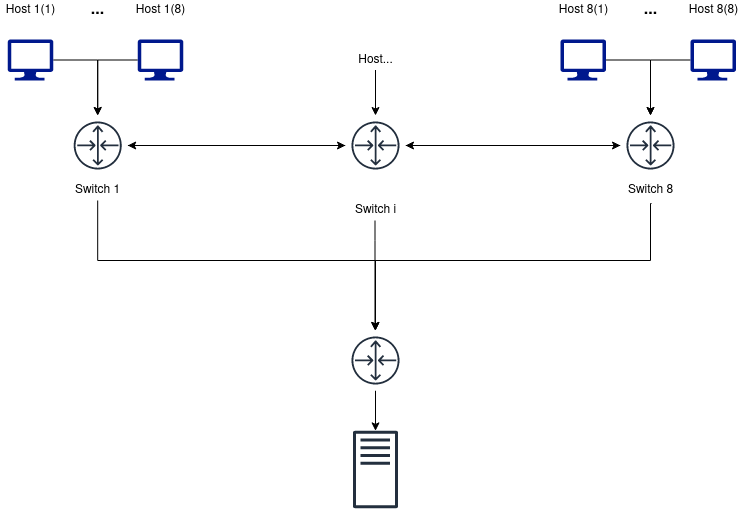
\includegraphics[width=0.8\textwidth]{images/DDoS}
	\caption{Distributed Denial of Service Network Topology}
	\label{fig:ddosNetwork}
\end{figure}

Within this topology, any number of hosts can be used to launch the distributed
denial of service attack. The topology is again implemented using the Mininet
Python API as follows:

\begin{lstlisting}[language=python, caption=DDoS Simulation Network Topology]
class LineTopo( Topo ):
    "Linear topology example."

    def __init__( self ):
        "Create linear topology"
        super(LineTopo, self).__init__()
        h1 = []
        h2 = []
        h3 = []
        h4 = []
        h5 = []
        h6 = []
        h7 = []
        h8 = []
        s = []		# list of switches
        server = []

        M=9
        N=8
        # add N hosts  h1..hN
        for i in range(1,N+1):
           h1.append(self.addHost('h1' + str(i)))
           h2.append(self.addHost('h2' + str(i)))
           h3.append(self.addHost('h3' + str(i)))
           h4.append(self.addHost('h4' + str(i)))
           h5.append(self.addHost('h5' + str(i)))
           h6.append(self.addHost('h6' + str(i)))
           h7.append(self.addHost('h7' + str(i)))
           h8.append(self.addHost('h8' + str(i)))

        # add N switches s1..sN
        for i in range(1,M+1):
           s.append(self.addSwitch('s' + str(i)))

	# add target server
        server.append(self.addHost('server'))

        # Add links from hi to si
        for i in range(N):
           self.addLink(h1[i], s[0])
           self.addLink(h2[i], s[1])
           self.addLink(h3[i], s[2])
           self.addLink(h4[i], s[3])
           self.addLink(h5[i], s[4])
           self.addLink(h6[i], s[5])
           self.addLink(h7[i], s[6])
           self.addLink(h8[i], s[7])

	# Add links from target server to s8
        self.addLink(server[0], s[8], cls=TCLink, bw=1000)

        # link switches
        for i in range(M-2):
           self.addLink(s[i],s[i+1])

        # link all switches to target switch
        for i in range(M-2):
            self.addLink(s[i], s[M-1])


topos = { 'mytopo': (lambda: LineTopo() ) }
\end{lstlisting}

Attacks are implemented as outlined in Section 3, however multiple nodes are
used for each attack. It was chosen to have all hosts from h11 to h44 to
participate in the attacks in order to generate a large enough volume of traffic
to cause a denial of service with a link bandwidth of 1Gbps on the link between
the server and it's adjacent switch.

In the case of the Distributed Denial of Service attack, no mitigation
techniques were implemented. The SDN NACL implementation could be implemented by
blacklisting each of the attacking nodes, however this would lead to a large
number of rules. Alternatively, utilising CIDR notation, as the attacking nodes
are sequential, a block could be blacklisted, however this would not have been a
realistic implementation for this simulation setup. Had individual subnets been
created for each grouping of 8 hosts, these subnets could have been determined
to be participating in the attack, and the entire subnet range blacklisted.
